\section{Iterative Model Update}
In this section, we describe how we iteratively update a dirty model based on
a cleaned batch of data.
We will show that this model update procedure can be interpreted as a Stochastic 
Gradient Descent (SGD) algorithm, which gives us a theoretical framework to analyze
convergence and bound the error at each step.
This theoretical framework will also inform how we should 

\subsection{Model Update Problem}
Suppose we have a cleaned batch of data $S_{clean}$ with features and labels $(X_{clean},Y_{clean})$, and a dirty model $\theta^{(d)}$. 
In the model update problem, we update the dirty model with some function $f(\cdot)$ i.e.,:
\[
\theta^{new} \leftarrow f(X_{clean},Y_{clean},\theta^{(d)})
\]
Our goal is that these updates should minimize the error the updated model and the true model $\theta^{(c)}$ (if we cleaned and trained over the entire data):
\[
error(\theta^{new}) = \| \theta^{new} - \theta^{(c)} \|
\]

\subsubsection{Naive Solutions}
We will explain why this problem neccesitates a new approach as existing techniques will not do what we want.
If we look at the progressive data cleaning problem in the abstract.
The first solution to this problem is to clean a sample of data, write this sample back, and then retrain the model on the partially cleaned data.
In fact, if we were to use current data cleaning architectures unmodified this is what they would do.
While this solution is guaranteed to be asympotically consistent (i.e., if we clean all the data we are guaranteed the correct solution), the performance of intermediate models can be very unreliable.
In statistics, there is a well-known phenomenon called Simpsons paradox, where mixtures of different populations of data can actually result in reversed trends.

So if mixing dirty and clean data is not the correct solution, the next approach would be to neglect the dirty data altogether.
We could recompute the model on only the cleaned data.
This solution is also guaranteed to be consistent, and intermediate results only reflect the clean data.
However, the problem here is that high-dimensional models are very sensitive to the sample size.
If our cleaning budget is small, sampling errors will dominate any reductions in data error.
We summarize these two approaches in Figure \ref{update-arch1}.

\begin{figure}[ht!]
\centering
 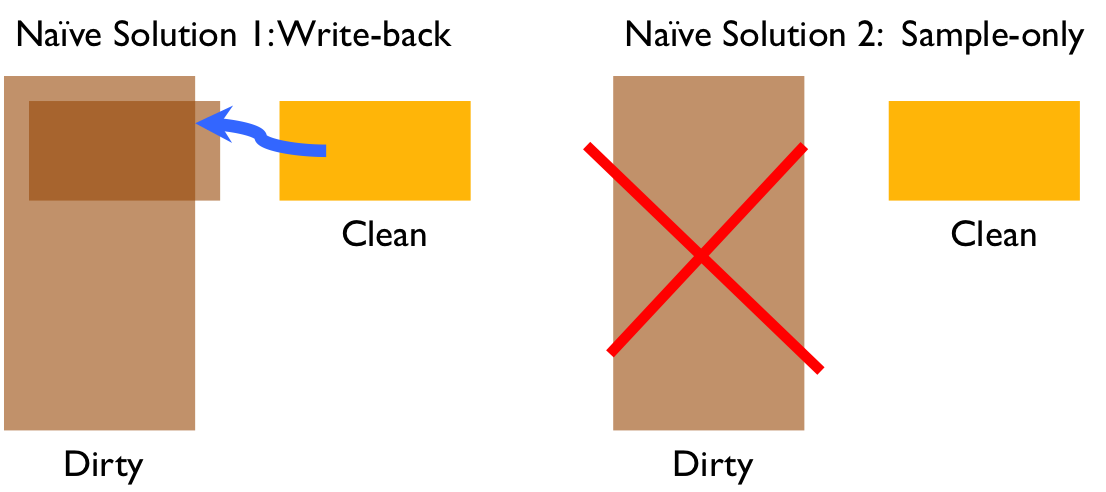
\includegraphics[width=\columnwidth]{figs/update-arch.png}
 \caption{The two naive solutions to the problem: writing-back the cleaned data, and training only on the sample. Writing back to the cleaned data potentially creates unreliable mixtures of data, and training only on the sample creates an issue of dimensionality and sample size. \label{update-arch1}}
\end{figure}

\subsection{Exploiting the Model's Geometry}
\sys addresses the update problem by using the model's geometry.
We restrict the class of Machine Learning models to convex regularized loss problems.
That is, as we vary the model $\theta$ the loss is bowl-shaped (Visualized in Figure \ref{update-arch2}a).
The model update problem can be visualized as follows.
We have a model $\theta^{(d)}$ (visualized in red) that is suboptimal with respect to the clean data.
We want to get to the optimal clean model $\theta^{(c)}$ which is visualized as a yellow star.

\begin{figure}[ht!]
\centering
 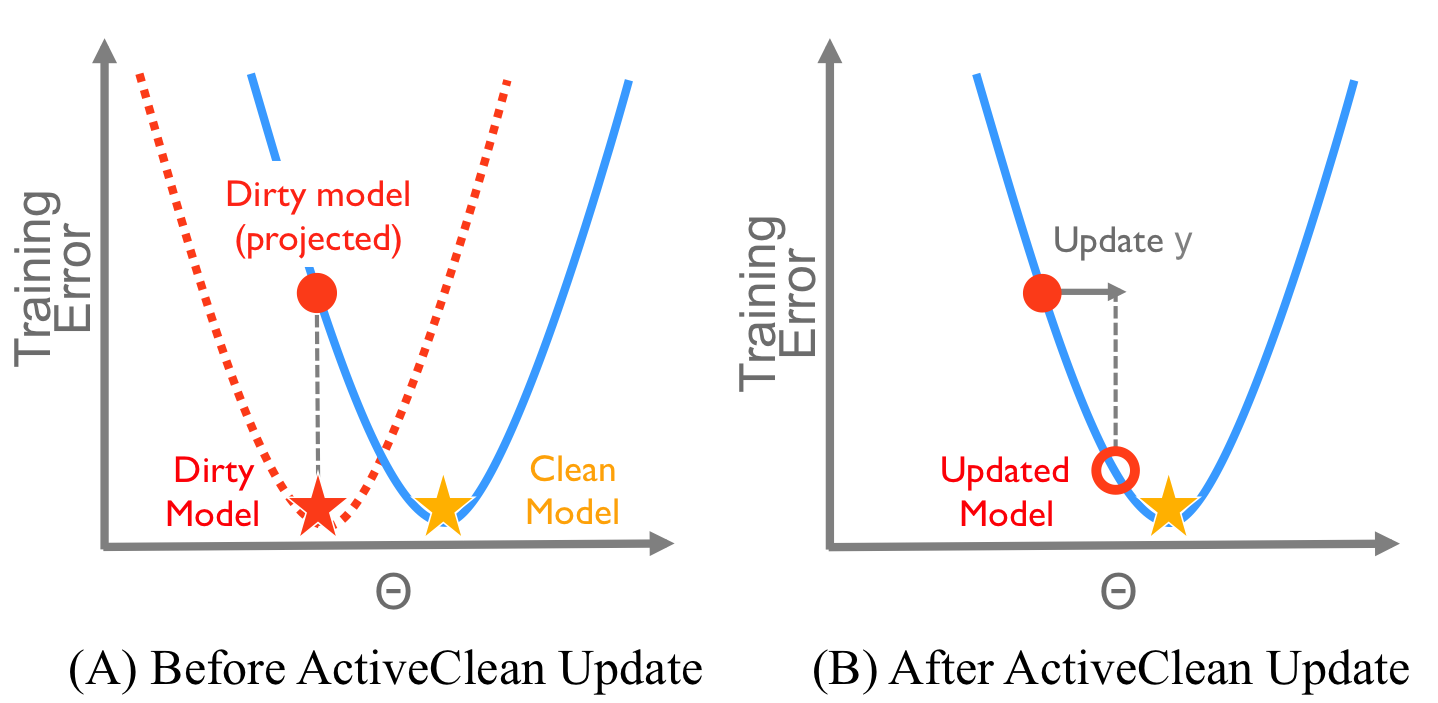
\includegraphics[width=\columnwidth]{figs/update-arch2.png}
 \caption{In \sys, we explore an important class of Machine Learning problems where the loss function (i.e., training error) varies convexly. A stale model can be thought of as a sub-optimal point and we want to move towards the optimal point. \label{update-arch2}}
\end{figure}

Ideally, we want an update that goes in the right direction along the loss curve (Figure \ref{update-arch2}b).
Mathematically, this direction corresponds to gradient of the loss with respect to $\theta$, and we need to move some distance $\gamma$ along this direction:
\[
\theta^{new} \leftarrow \theta^{(d)} - \gamma \cdot \nabla\phi(X_{clean},Y_{clean},\theta^{(d)})
\]
Let, $g_{S}(\theta) = \nabla\phi(X_{clean},Y_{clean},\theta)$, then for every batch of data cleaned, we apply the update to the current best model estimate:
\[
\theta^{(t)} \leftarrow \theta^{(t-1)} - \gamma \cdot g_{S}(\theta^{(t-1)}) \blacksquare
\]

Here, we can draw an analogy to Materialized View maintenance, since after all, a model parameterized by $\theta$ is just a table of floating point numbers.
Krishnan et al. proposed a technique called sample view cleaning, in which they take a clean sample of data and propogate the updates to a Materialized View.
Similarly, in this work, we take the information from a sample of cleaned data and propagate an update with the gradient.
The insight that many mathematical problems are analogous to view maintenance has recently been noted others as well \cite{nikolic2014linview}. 

\subsubsection{Selecting the Parameters}
The proposed update policy makes theoretical and intuitive sense for convex loss problems.
However, there are a few issues that we need to sort out to make this a pratical and meaningful update.

\vspace{0.5em}

\noindent\textbf{Step Size $\gamma$ : } The first problem is that we have not explained how to pick the step size $\gamma$. In other words, how far should we travel in the gradient direction.

\vspace{0.5em}

\noindent\textbf{Choosing $S$: } The next problem is that the optimal clean model depends on \emph{all} the clean data, not just a sample. 
So $g_S$ is really an approximation of the gradient with some error $g^* \pm \epsilon$. 
The quality of the update depends on how well we can approximate $g^*$ using $g_S$.
The problem is how should we construct the sample of data to clean $S$ to get the most accurate update.

\subsection{Stochastic Gradient Descent}
This update policy can be formalized as a class of very well studied algorithms called Stochastic Gradient Descent.
This gives us a theoretical framework to understand and analyze our update rule, bound the error, and choosing points to clean.
Mini-batch stochastic gradient descent (SGD) is an algorithm for finding the optimal value
of $\theta$, given the convex loss, and data.
In SGD, we start with an abitrary initialization and iterate to convergence.
In our case, we start with an initialization which is the dirty model, the model trained completely on the dirty data.
Then, at each iteration we sample a mini-batch of data on which we apply our expensive data cleaning operations.
The update rules in SGD mirror our update policy:
 \[
 \theta^{(t+1)}\leftarrow\theta^{(t)}-\gamma\frac{1}{\mid S^{(t)}\mid}\sum_{i\in S^{(t)}}g_S
 \]

\vspace{0.5em}

\noindent\textbf{ Setting $\gamma$: } There is extensive literature in machine learning for choosing $\gamma$ appropriately. $\gamma$ can be set either to be a constant or decayed over time. Many machine learning frameworks (e.g., MLLib, Sci-kit Learn, Vowpal Wabbit) automatically set learning rates or provide different learning scheduling frameworks. 
In our experiments, we use a technique called inverse scaling where there is a parameter $\gamma_0=0.1$, and at each iteration we reduce it to $\gamma_t = \frac{\gamma_0}{\mid S \mid t}$. 

\vspace{0.5em}

\noindent\textbf{ Convergence: } The next property of concern is convergence. Convergence properties of batch SGD formulations has been well studied \cite{dekel2012optimal}. 
The conditions on this convergence are essentially that at each step the estimate of the gradient $g_S$ has to be unbiased, that is on average correct. 

\begin{proposition}
For an appropriately chosen learning rate $\gamma_t$, batch stochastic gradient descent will converge if $\mathbb{E}(g_S)=g^*$.
\label{unbiased}
\end{proposition}

A direct result of convergence is a guarantee on statistical consistency.
Another interesting consequence of this result is that we can sample $S$ in any way that we want
as long as our estimate in unbiased.

\vspace{0.5em}

\noindent\textbf{ Convergence Rate: } The convergence rates of SGD are also well analyzed \cite{dekel2012optimal,bertsekas2011incremental,zhao2014stochastic}. 
Suppose, a user cleans a batch size of $b$ examples at each iteration.
This allows us to bound the error of intermediate models and understand the expected number of steps before a model within a certain error. 

\begin{proposition}
For a general convex loss, a batch size $b$, and $t$ iterations, the convergence rate is bounded by $O(\frac{\sigma^2}{\sqrt{bt}})$. 
$\sigma^2$ is the variance in the estimate of the gradient at each iteration:
\[
\mathbb{E}(\|g_S - g^*\|^2)
\]
\end{proposition}

There is an interesting tradeoff between batch size an convergence rate.
Increasing the batch size reduces the variance $\sigma^2$, however it does
mean at each iteration you are doing more work.
In a data cleaning context, this is a problem since the bottlneck is the work at 
each iteration not the number of iterations.

\subsection{Reducing the Variance $\sigma^2$}\label{dist-samp}
In the Machine Learning and Optimization literature, SGD algorithms are optimized to avoid scanning the entire data.
Uniform sampling is cheap so it is the preferred solution.
However, there are a few observations about the data cleaning problem that suggest that we can do better if we carefuly select which points to clean.
The key property that we need to preserve is unbiasedness (Proposition \ref{unbiased}).

\vspace{0.5em}

\noindent\textbf{Observation 1. Detection vs. Cleaning: } In many applications, enumerating the set of corrupted records is much easier than cleaning them. For example, we may be able to select the set of rows that have missing values but actually filling those missing values is expensive. Likewise, in the constraint literature, selecting a set of rows that have a violated constraint can be done in polynomial time, however, fixing the constraints is NP-Hard.
In other words, cleaning a batch of data can be far more expensive than a scan.
We can use this to our advantage to reduce the variance of the gradient without affecting our batch size.

We first select a set of records before starting we select a set of dirty records $R_{dirty} \subseteq R$. 
We construct batch $S_{dirty}$ only from the dirty records and apply cleaning to this batch.
Now the problem is that this sample (and the resulting gradient) is possibly biased since we are excluding some data.
However, since we know that the set $R - R_{dirty}$ is clean, we can compute the average gradient over those records without cleaning:
\[
g_c(\theta^{t}) = \frac{1}{\mid R - R_{dirty} \mid} \sum g_i(\theta^{t})
\]
Since we know the partition sizes, we can combine the two estimates $g_c$ and $g_S$ togther:
\[
g(\theta^{t}) = \frac{\mid R_{dirty} \mid g_S + \mid R - R_{dirty} \mid g_c \mid }{\mid R \mid} \blacksquare
\]

\begin{lemma}
The gradient estimate $g(\theta^{t})$ is unbiased if $g_S$ is an unbiased estimate of:
\[
\frac{1}{\mid R_{dirty} \mid} \sum g_i(\theta^{t})
\]
\end{lemma}
\begin{proof}[Sketch]
This result follows directly from the linearity of expectation, since we are adding a deterministic result with an unbiased result.
\end{proof}

\vspace{0.5em}

\noindent\textbf{Observation 2. Pre-processing is relatively cheap: }
Data cleaning is often the most expensive step in the workflow, so optimizing for scan cost may lead to neglible overall time improvements.
We can sacrifice a small overhead in pre-computation for each data point to determine its value to the model and select a sampling distribution accordingly.
Intuitively, while each iteration has an increased cost, it also makes more progress towards the optimum.

In our problem, we are trying to select a sample $S_{dirty}$ from $R_{dirty}$.
If we sample every element $i \in R_{dirty}$ with probability $p_i$, the question is
how can we compute a set of $\{p_i\}$ such that variance of the gradient $\sigma^2$ is minimized. 


\subsection{Summary}
In summary, while we still have to discuss how we find the estimator function $e(\cdot)$, we can describe the basic processing workflow of \sys.
\begin{enumerate}[noitemsep]
\item Initialize with $\theta^{(0)}$ as the dirty model, $T$ iterations, with a batch size $B$
\item For rounds i=1...T
\begin{enumerate}
	\item Sample $B$ candidate dirty data points with probabilites as described.
	\item Apply data cleaning to the sample of data.
	\item Apply weighted gradient descent to update the model.
\end{enumerate}
\item Return $\theta^{(T)}$
\end{enumerate} 